\documentclass[twocolumn, 11pt]{scrartcl}
\usepackage[narrow-margins]{jamiepack}
\addbibresource{bib.bib}

\title{Elliptic Curve Codes}
\author{Jamie Low \& Oliver Ang}

% Uncomment to check spacing
\raggedbottom

\begin{document}

% This is for \maketitle
\title{\textbf{Elliptic Curve Codes: Recent Constructions and Isogeny-Induced Transformations}}
\author{\textbf{Jamie Low Jiaqi \& Oliver Ang Wei Jie}\\School of Physical and Mathematical Sciences, Nanyang Technological University, Singapore}
\date{MH4310 Coding Theory, Semester 1, Academic Year 2026--2027}
\maketitle

% These are for the page headers
\title{Elliptic Curve Codes}
\author{Jamie Low \& Oliver Ang}
\date{}

\usection{Abstract}

Elliptic curves are the only algebraic curves whose points admit a canonical group structure. Algebraic geometry code constructions using elliptic curves can therefore exploit the group law to obtain better parameters and properties. This report introduces the machinery behind elliptic curve codes and surveys recent constructions of MDS elliptic curve codes. As a novel direction, we also explore how isogenies interact with elliptic codes and their parameters, culminating in a new family of quasi-cyclic MDS codes.

\section{Introduction} \label{section:introduction}

Algebraic geometry (AG) codes are a family of linear error-correcting codes introduced by Valeriy Goppa in the early 1980s \cite{goppa1983algebraico}. Broadly speaking, they are defined by evaluating rational functions on an algebraic curve $\mcC/\bbF_q$ at some set of evaluation points. They generalise the widely used Generalised Reed--Solomon (GRS) codes \cite{macwilliams1977theory}, which are obtained by letting $\mcC$ be the projective line $\bbP^1(\bbF_q)$, which has genus 0.

The code parameters are closely related to the geometry of the chosen curve, particularly its genus and the number of rational points. AG codes therefore provide a natural connection between algebraic geometry and coding theory. In 1982, Tsfasman, Vl\u{a}du\c{t} and Zink took this idea further, using curves with many rational points to construct the first code families whose asymptotic parameters surpass the Gilbert--Varshamov bound \cite{tsfasman1982modular}, demonstrating the ability for algebraic geometry to produce asymptotically good codes and sparking further research of AG codes constructed from a diverse range of algebraic curves.

The simplest AG codes inequivalent to GRS codes arise from elliptic curves, which are smooth projective curves of genus 1. They are the only algebraic curves whose points admit a canonical abelian group structure \cite[\S X.3]{silverman2009arithmetic}.\footnote{Provided they have an $\bbF_q$-rational point, elliptic curves are the only algebraic curves isomorphic to their own Jacobians and hence are abelian varieties.} AG codes defined using elliptic curves are called elliptic curve codes, or simply elliptic codes. Using the group structure, algebraic constructions unique to genus 1 have been discovered, yielding codes with better parameters (e.g. maximum distance separable (MDS) codes) and desirable properties like iso-duality, with applications in quantum error correction. The group structure also supplies arguments for proving bounds on code parameters.

Elliptic curves also carry isogenies, which are curve morphisms preserving the group structure. Isogenies are heavily used in post-quantum cryptography \cite{jamielow2027,basso2026prism,NISTPQC-ADD-R3:SQIsign26}, but their applications to coding theory remain largely unexplored. We embark on an AI-assisted project, using Claude and SageMath to explore the different ways in which isogenies can transform an elliptic curve's function field, and hence the parameters of an elliptic code.

The goal of our report is to explain how the remarkable properties of elliptic curves yield unique and excellent constructions of elliptic codes that stand out from general AG codes. In \Cref{section:preliminaries,section:ecc}, we introduce elliptic codes as a concrete and accessible instance of AG codes by developing the necessary background underlying the arithmetic of elliptic curves and elliptic codes. We then survey recent constructions and bounds in \Cref{section:group-law,section:mds-ecc}. We conclude with a documentation of our exploration on the interaction between isogenies and elliptic codes in \Cref{section:isogenies}.

\section{Preliminaries} \label{section:preliminaries}

We summarise key definitions and results pertaining to elliptic curves and elliptic codes. For a more detailed description with proofs of results, we refer the reader to the following comprehensive standard references, which our exposition is based on:
\begin{itemize}[itemsep=-8pt]
    \item Silverman's book \cite{silverman2009arithmetic} for basic arithmetic geometry, with a focus on elliptic curves;
    \item Stichtenoth's book \cite{stichtenoth2009algebraic} for algebraic function fields and algebraic geometry (AG) codes.
\end{itemize}
Henceforth, let $q=p^m$ denote a prime power.

An \textbf{elliptic curve} $\mcE$ over $\bbF_q$ is a smooth projective curve of genus 1. Equivalently, $\mcE$ is the set of points $(x,y)\in\Fbar{q}^2$ satisfying an equation of the form
\[ y^2+a_1xy+a_3y=x^3+a_2x^2+a_4x+a_6, \quad a_i\in\bbF_q \eqlabel{eqn:ec} \]
together with a point at infinity $\infty$, provided that no point is singular. A point $P\in\mcE$ is \textbf{$\bbF_q$-rational} if $P\in\bbF_q^2\cup\set\infty$. The set of $\bbF_q$-rational points is denoted by $\mcE(\bbF_q)$, and the set $\mcE(\bbF_q)\bs\set\infty$ of affine $\bbF_q$-rational points by $\mcE(\bbF_q)^*$. Its cardinality is constrained by the Hasse--Weil bound \cite[\S V.1]{silverman2009arithmetic}
\[ \abs{\#\mcE(\bbF_q)-(q+1)}\leq\floor{2\sqrt q}. \]
The points of $\mcE$ form an abelian group $(\mcE,\oplus)$ with identity $\infty$, where the group addition $\oplus$ is governed by the equations in \cite[\S III.2]{silverman2009arithmetic} and visualised in \Cref{fig:elliptic-group-law}. As is standard in the literature, $[m]P$ denotes the $m$-fold sum $P\oplus\cdots\oplus P$ for $m\in\bbN$, and $[-m]P:=\ominus[m]P$.

\begin{figure}
    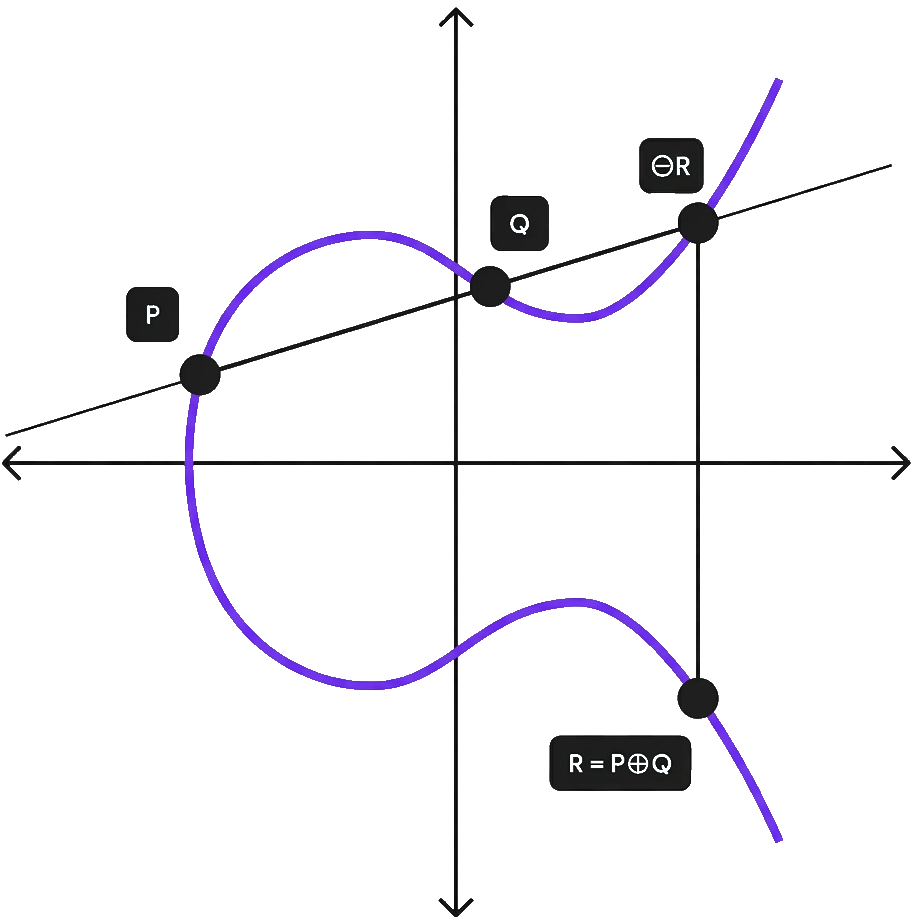
\includegraphics[width=0.3\textwidth]{assets/elliptic-group-law}
    \figcaption{The group law of an elliptic curve $\mcE$ over $\bbR$ \cite{elusiv_ecc_2023}}
    \label[figure]{fig:elliptic-group-law}
\end{figure}

A \textbf{divisor} of $\mcE$ is an element $D$ of the free abelian group $\Div\mcE=\bbZ[\mcE]$ over the points of $\mcE$. In other words, it is a formal sum
\[ D=\sum_{P\in\mcE} n_P\cdot(P),\quad n_P\in\bbZ \]
where all but finitely many $n_P$ are zero. Its \textbf{support} and \textbf{degree} are, respectively,
\[ \supp D=\set{P\in\mcE:n_P\neq0} \qand \deg D=\sum_{P\in\mcE} n_P. \]
Its \textbf{sum} is the evaluation of the formal sum using the elliptic group law, and is denoted by
\[ \Sigma(D)=\bigoplus_{P\in\mcE} [n_P]P. \]
A partial ordering on $\Div\mcE$ is defined by
\[ \sum_{P\in\mcE} n_P(P)\leq\sum_{P\in\mcE} n'_P(P) \qiff \forall P\in\mcE:\quad n_P\leq n'_P. \]
The \textbf{function field} $\bbF_q(\mcE)$ of $\mcE$ is the field $\bbF_q(x,y)$, where $x$ is transcendental over $\bbF_q$ and $y$ is algebraic over $\bbF_q(x)$ subject to \Cref{eqn:ec}. For $f\in\bbF_q(\mcE)$, set
\[ \div f:=\sum_{P\in\mcE} \ord_P(f)\cdot(P),\quad\text{where} \]
\begin{itemize}[itemsep=-8pt]
    \item $\ord_P(f)=n\in\bbZ^+$ if $f$ has a zero of order $n$ at $P$;
    \item $\ord_P(f)=-n\in\bbZ^-$ if $f$ has a pole of order $n$ at $P$;
    \item $\ord_P(f)=0$ otherwise.
\end{itemize}
Such divisors are called \textbf{principal} and form a subgroup $\PDiv\mcE$ of the degree-0 divisors $\Div^0\mcE$. Two divisors (of any degree) are called \textbf{equivalent} if they differ by a principal divisor. The \textbf{Jacobian} of $\mcE$ is the quotient $\Jac\mcE:=\Div^0\mcE/\PDiv\mcE$, which is famously isomorphic to $\mcE$ (cf. \Cref{section:group-law}).\footnote{More precisely, this quotient is called the Picard group of degree 0, but this is isomorphic to the Jacobian variety.}

Given a divisor $G\in\Div\mcE$, we construct the \textbf{Riemann--Roch space}
\[ \mcL(G):=\set{f\in\bbF_q(\mcE)^*:\div f\geq-G}\cup\set0. \]
This is a finite-dimensional vector subspace of $\bbF_q(\mcE)$, and we denote its dimension by $\ell(G)$. For elliptic curves, the Riemann--Roch Theorem \cite[\S1.5]{stichtenoth2009algebraic} gives us $\ell(G)\geq\deg G$, with equality when $\deg G\geq1$.

The \textbf{space of differential forms} $\Omega_\mcE$ on $\mcE$ is the $\bbF_q$-vector space generated by symbols of the form $\df$ for $f\in\bbF_q(\mcE)$, subject to the relations
\[ \dx[(f+g)]=\df+\dg,\quad \dx[(fg)]=f\,\dg+g\,\df,\quad \da=0 \]
for all $f,g\in\bbF_q(\mcE)$ and $a\in\bbF_q$. Around a point $P\in\mcE$, every $\omega\in\Omega_\mcE^*$ can be written uniquely as
\[ \omega=\sum_{n=m}^\infty a_nt^n\dt\quad\text{for some  } \begin{cases}
        t\in\bbF_q(\mcE),\ \ord_P(t)=1, \\
        a_n\in\bbF_q,\ a_m\neq 0,\ m\in\bbZ.
    \end{cases} \]
For $\omega\in\Omega_\mcE^*$, set $\ord_P(\omega):=m$, $\Res_P(\omega):=a_{-1}$ (or 0 if $m\geq 0$),
\vspace{-9pt}
\begin{align*}
    \div\omega&:=\sum_{P\in\mcE}\;\ord_P(\omega)\cdot(P),\quad\text{and}\\
    \Omega(G)&:=\set{\omega\in\Omega_\mcE^*:\div\omega\geq G}\cup\set0.
\end{align*}
The divisors $\div\omega$ are called \textbf{canonical}. In genus 1, the sets of canonical and principal divisors coincide \cite[Cor.~1.4.12]{stichtenoth2009algebraic}.

\section{Elliptic codes} \label{section:ecc}

This section introduces general elliptic codes, their parameters, and their encoding and decoding mechanisms. In later sections, we consider specialised codes with better properties.

Let $n\in\bbZ^+$, $\mcE$ be an elliptic curve and $D,G\in\Div\mcE$ be two divisors such that $1\leq\deg G\leq n-1$, $\supp D\cap\supp G=\emptyset$, and $D=(P_1)+\cdots+(P_n)$ is a sum of $n$ distinct $\bbF_q$-rational points. We adopt the notation
\[ f(D):=(f(P_1),\hdots,f(P_n))\in\bbF_q^n\qtx{for}f\in\mcL(G). \]
Construct an ordered basis $(\varphi_1,\hdots,\varphi_k)$ of $\mcL(G)$, where $k=\ell(G)=\deg G$ by Riemann--Roch. Then, there exists an $[n,k,d]_q$ code
\[ C_\mcL(D,G):=\set{f(D):f\in\mcL(G)}=\ang{\varphi_1(D),\hdots,\varphi_k(D)}, \]
which encodes a message $\bfm\in\bbF_q^k$ as $\sum_{i=1}^k m_i\varphi_i(D)$.

The quantity $d^*:=\deg(D-G)=n-k$ is called the \textbf{designed distance} of $C_\mcL(D,G)$. The code has minimum distance $d\geq d^*$ \cite[\S2]{stichtenoth2009algebraic}, so the Singleton defect is at most 1. We will see in \Cref{section:mds-ecc} ways to construct MDS elliptic codes.

The Euclidean dual code $C_\mcL(D,G)^{\perp_\rmE}$ of $C_\mcL(D,G)$ is
\[ C_\Omega(D,G)=\set*{(\Res_{P_1}(\omega),\hdots,\Res_{P_n}(\omega)):\omega\in\Omega(G-D)}, \]
as proven in \cite[Prop.~8]{o2008key}. Choose $t\in\bbF_q(\mcE)$ such that $\ord_{P_i}(t)=1$ for $1\leq i\leq n$. Then, the differential $\eta:=\dt/t$ has the property that every $\omega\in\Omega(G-D)$ can be written as $f\eta$ for some $f\in\mcL(H)$, where $H=D-G+\div\eta$ \cite[\S8.1]{stichtenoth2009algebraic}. As such, we have the beautiful result that $C_\Omega(D,G)=C_\mcL(D,H)$. Consequently, $C_\mcL(D,G)$ is either MDS or near-MDS.

Common choices of $G$ include $G=k(Q)$ for some $Q\in\mcE$, or $G=(k-1)(P)+(Q)$ for some $P,Q\in\mcE$. Such codes are called \textbf{one-point codes} and \textbf{two-point codes} respectively. The former has the advantage that a basis of $\mcL(G)$ is easy to construct.

\subsection{Decoding}

The remainder of this section is devoted to decoding. We illustrate one relatively simple (but suboptimal) decoding algorithm \cite[\S6.2]{hoholdt1998algebraic}\footnote{This algorithm applies to curves of arbitrary genera and does not use the group law. There are better algorithms \cite{hoholdt1995decoding,o2008key}, but we select this one for pedagogical reasons.} for the $[n,n-k,\geq\!k]$ code $C:=C_\Omega(D,k(Q))$, the dual of a one-point code.

Denote by $R=\bigcup_{m=1}^\infty \mcL(m(Q))$ the $\bbF_q$-vector space of functions having no poles away from $Q$. Let $(\varphi_j)_{j\in\bbZ^+}$ be a basis for $R$, ordered such that $\varphi_1=1$ and $\ord_Q(\varphi_j)=-j$ for $j\geq2$, so that $\mcL(m(Q))=\ang{\varphi_1,\hdots,\varphi_m}$. For instance, if $Q=\infty$, we may take the basis $(1,x,y,x^2,xy,x^3,x^2y,\hdots)$.

Let $\bfr=\bfc+\bfe\in\bbF_q^n$ be a received word, where $\bfc\in C$ and $\bfe\in\bbF_q^n$ are an unknown codeword and error respectively. Define the \textbf{syndrome functional}
\[ S:\mcL(G)\to\bbF_q, \quad f\mapsto\bfr\dotpr f(D). \]
Let $f,g\in\mcL(s(Q))\subset\mcL(G)$, where $s=\floor{k/2}$, so that $fg\in\mcL(G)$. Since $(fg)(D)\in C_\mcL(D,G)=C^\perp$, we have $\bfc\dotpr (fg)(D)=0$, and so
\[ S(fg)=(\bfc+\bfe)\dotpr (fg)(D)=\sum_{i\in\supp\bfe} e_if(P_i)g(P_i). \]

\vspace{-1.9em}
Hence, the space
\[ K=\set[\big]{f\in\mcL(s(Q)):S(fg)=0\ \forall g\in \mcL(s(Q))} \]
contains the functions $f$ vanishing at $\supp\bfe$, and thus, reveals the error positions. Sampling $f\in K^*$, the coordinate set $I$ where $f$ vanishes contains $\supp\bfe$. As $S$ is linear, it suffices to consider $S(\varphi_i\varphi_j)$ for $1\leq i,j\leq s$.

Finally, we use \cite[Prop.~6.1]{o2008key} to find the error values. Assuming $\#I<d(C)$, $\bfe$ is the unique solution $\bfx$ of the system
\[ \bfx\dotpr f_i(D)=S(f_i)\quad\forall 1\leq i\leq k\qand x_i=0\quad\forall i\notin I. \]
\cite[Prop.~6.5]{o2008key} shows that this decoding algorithm can correct $\floor{k/2}-1$ errors (which is suboptimal if $C$ is MDS) with complexity $\mcO(n^3)$.

\begin{algorithm}{Basic Decoding \cite[\S6.2]{hoholdt1998algebraic}}{}
    \textbf{Input:} A received word $\bfr\in\bbF_q^n$
    
    \textbf{Output:} The decoded codeword $\bfc\in C_\Omega(D,G)$
    
    \textbf{Steps:}
    
    \begin{enumerate}[itemsep=-2pt]
        \item $\bfS\gets\br{S(\varphi_i\varphi_j)}_{i,j=1}^s\in\bbF_q^{s\times s}$
        \item $K\gets\ker\bfS$ \quad
        \item $f\gets\sum_{i=1}^s \lambda_i\varphi_i$ for some $\bm\lambda\in K^*$
        \item $I\gets\set{i:f(P_i)=0}$ \quad // Contains $\supp\bfe$
        \item $\bfH\gets[\varphi_1(D),\hdots,\varphi_k(D)]\in\bbF_q^{n\times k}$
        \item Let $\bfe$ be the unique (row) vector satisfying $\bfe\bfH=\bfr\bfH$ and $e_i=0$ for all $i\notin I$
        \item Return $\bfr-\bfe$
    \end{enumerate}
\end{algorithm}

\section{Exploiting the group law} \label{section:group-law}

Every smooth projective curve $\mcC$ of genus $g$ carries an abelian variety of dimension $g$, its Jacobian $\Jac\mcC$, whose points are the divisor classes of degree zero on $\mcC$ (cf. \Cref{section:preliminaries}). What distinguishes genus 1 is that the group structure can be transported from the Jacobian to the curve. Specifically, for an elliptic curve, the \textbf{Abel--Jacobi map}
\[ \mcE\lra\Jac\mcE, \qquad P\longmapsto\br{(P)-(\infty)} \]
is a bijection whose inverse is the sum map $\Sigma$ of \Cref{section:preliminaries}, and the group law it induces on $\mcE$ agrees with the geometric one in \cite[\S III.3]{silverman2009arithmetic}. This is the isomorphism with the Jacobian noted in the abstract.

In coding theory, one can exploit this group law to obtain better codes. For an AG code $C_\mcL(D,G)$ with $g=1$, the points in $D$ and $G$ lie in a group. Conditions on $D$ and $G$, which govern the code parameters, may therefore be rewritten as conditions on sums of these evaluation points using tools such as the Abel--Jacobi Theorem. For $g\geq2$ the group lives on a higher-dimensional variety, and no such translation is available.

\begin{lemma}{Abel--Jacobi \cite[Cor.~III.3.5]{silverman2009arithmetic}}{abel-jacobi}
    $A\in\Div^0\mcE$ is principal if and only if $\Sigma(A)=\infty$.
\end{lemma}

Henceforth we assume, as is standard, that $\supp G\subset\mcE(\bbF_q)$, so that $\Sigma(G)\in\mcE(\bbF_q)$. \Cref{section:ecc} established that an elliptic code is either MDS or near-MDS. The following criterion decides which.

\begin{theorem}{Subset-sum criterion \cite{munuera1993mds,li2015minimum}}{mds-criterion}
    Let $C_\mcL(D,G)$ be as in \Cref{section:ecc}, with $D=(P_1)+\cdots+(P_n)$ and $k=\deg G$. Then $d=n-k$ if and only if there are $k$ distinct points $P_{i_1},\hdots,P_{i_k}\in\supp D$ with
    \[ P_{i_1}\oplus\cdots\oplus P_{i_k}=\Sigma(G). \eqlabel{eqn:mds-criterion} \]
    Otherwise, $d=n-k+1$, and the code is MDS.
\end{theorem}

The criterion is more than a test, since its proof is constructive and hands us the minimum-weight codewords explicitly. Suppose $S=\set{P_{i_1},\hdots,P_{i_k}}\subseteq\supp D$ satisfies \Cref{eqn:mds-criterion}. The divisor $\sum_{P\in S}(P)-G$ then has degree 0 and sum $\infty$, so \Cref{lemma:abel-jacobi} produces a function $f$ with $\div f=\sum_{P\in S}(P)-G$. This $f$ lies in $\mcL(G)$ and vanishes on $S$ and nowhere else in $\supp D$, so $f(D)$ is a codeword of weight exactly $n-k$. Two functions with the same divisor differ by a constant, and distinct subsets give codewords with distinct supports, so we obtain every minimum-weight codeword exactly once up to scaling. Writing $A_{n-k}$ for the number of codewords of weight $n-k$,
\begin{align*}
A_{n-k}&=(q-1)\cdot\#\mcS,\quad\text{where} \\
\mcS&=\set*{S\subseteq\supp D:\#S=k,\ \textstyle\bigoplus_{P\in S} P=\Sigma(G)}.
\end{align*}
Counting the codewords of a given weight is hard in general. Here the group law reduces it to counting the solutions of a subset-sum problem in $\mcE(\bbF_q)$, which is the form in which the minimum distance of elliptic codes is usually studied \cite{li2015minimum}.

A second consequence concerns the shape of $G$ itself. Replacing $G$ by an equivalent divisor yields an equivalent code. Hence, up to coordinate scalings, we may take $G$ to be supported on up to two points, which is the case for all constructions in this report.

\begin{lemma}{\cite[Prop.~2.2.14]{stichtenoth2009algebraic}}{equiv-codes}
    If $G$ and $H$ are equivalent divisors whose supports are disjoint from $D$, then $C_\mcL(D,G)$ and $C_\mcL(D,G')$ differ at most by coordinate scaling.
\end{lemma}

\begin{corollary}{Two-point normal form \cite{wang2025nonrs,zhu2026isodual}}{normal-form}
    Fix $D$ and $G$ as in \Cref{section:ecc}. Let $Q_0,Q_1\in\mcE(\bbF_q)\bs\supp D$ be such that $G':=(k-1)(Q_0)+(Q_1)$ satisfies $\Sigma(G')=\Sigma(G)$. Then $C_\mcL(D,G)$ and $C_\mcL(D,G')$ differ at most by coordinate scaling.
\end{corollary}

A third consequence is that the group law supplies the code with automorphisms. For $R\in\mcE(\bbF_q)$, the \textbf{translation} map $\tau_R:P\mapsto P\oplus R$ is an automorphism of $\mcE$ as a curve. It acts on functions by $\tau_R^*f=f\circ\tau_R$ and on divisors by $\tau_R^*(P)=(P\ominus R)$, so that $\tau_R^*\mcL(G)=\mcL(\tau_R^*G)$.

\begin{theorem}{Translation automorphisms \cite{ma2023automorphism}}{translations}
    Let $C:=C_\mcL(D,G)$ be as in \Cref{section:ecc}. Suppose $R\in\mcE(\bbF_q)$ satisfies $[k]R=\infty$ and $\supp D$ is stable under $\tau_R$.\footnote{The latter condition holds, for instance, when $\supp D$ is a subgroup of $\mcE(\bbF_q)$ containing $R$, as in \Cref{construction:index-two}.} Then $\tau_R$ induces a monomial automorphism of $C$.
\end{theorem}

Elliptic curves have many more curve automorphisms than other algebraic curves \cite{ma2023automorphism,stichtenoth1973automorphism}, so elliptic codes generally have many more code automorphisms than other AG codes. They have been used in \cite{tong2013quasicyclic,ma2023automorphism}, for instance, and have potential applications in decoding and determining weight distributions.

\mycomment{
These automorphisms are a feature of genus 1. Denote by $\Aut(\mcE,\infty)$ the subgroup of automorphisms fixing $\infty$, which has cardinality dividing 24 \cite[Thm.~III.10.1]{silverman2009arithmetic}. Then, the automorphism group of $\mcE$ as a curve is $\Aut\mcE=\mcE(\bbF_q)\rtimes\Aut(\mcE,\infty)$ \cite{ma2023automorphism}, which has cardinality $\mcO(q)$. For a curve $\mcC$ of genus $g\geq 2$, $\#\Aut\mcC$ is bounded in terms of $g$ alone, with $\#\Aut\mcC<16g^4$ unless $\mcC$ is a Hermitian curve \cite{stichtenoth1973automorphism}, so for fixed genus, it cannot keep pace with the number of rational points as $q$ grows. As applications, Tong and Ding build quasi-cyclic near-MDS codes from elliptic curves using $\Aut(\mcE,\infty)$ \cite{tong2013quasicyclic}, while Ma and Xing construct optimal locally repairable codes using $\Aut\mcE$ \cite{ma2023automorphism}.
}

\section{MDS elliptic codes} \label{section:mds-ecc}

To determine whether a given AG code is MDS, one usually studies the vanishing of rational functions via Riemann--Roch computations. For $g=1$, it becomes a purely combinatorial question on a finite abelian group, since $C_\mcL(D,G)$ is MDS precisely when no $k$-element subset of $\supp D$ sums to $\Sigma(G)$. This section surveys constructions that arrange $D$ and $G$ so that this holds, and then asks how long such a code can be.

Elliptic curves were introduced in order to escape the length restriction on GRS codes, for which $n\leq q+1$. By the Hasse--Weil bound (cf. \Cref{section:preliminaries}), $\mcE(\bbF_q)$ may contain as many as $M:=q+1+\floor{2\sqrt q}$ points. Being MDS, however, is expensive. As $\supp D$ grows, some $k$-subset of it is eventually forced to sum to $\Sigma(G)$, whence \Cref{theorem:mds-criterion} precludes the MDS property. We shall see below that an MDS elliptic code cannot use more than roughly half of the available rational points. The full length $n\approx q+2\sqrt q$ is available only to near-MDS codes.

\subsection{Constructions}

The simplest way to obtain the condition of \Cref{theorem:mds-criterion} is a parity argument on a one-point code. Suppose $N:=\#\mcE(\bbF_q)$ is even and let $H\leq\mcE(\bbF_q)$ be a subgroup of index 2, so that $\mcE(\bbF_q)=H\sqcup(Q\oplus H)$ for any $Q\notin H$. Sums then behave predictably, as $k$ elements of $H$ sum into $H$, while $k$ elements of $Q\oplus H$ sum into $H$ or $Q\oplus H$ according to the parity of $k$.

\begin{construction}{Index-two codes \cite{wang2025nonrs}}{index-two}
    Let $N=\#\mcE(\bbF_q)$ be even and let $H\leq\mcE(\bbF_q)$ be a subgroup of index 2. Choose $Q\in\mcE(\bbF_q)\setminus H$.
    \begin{enumerate}[label={(\alph*)}, left=-4pt, topsep=2pt, itemsep=0pt]
        \item If $k$ is odd, set $D=\sum_{P\in H}(P)$ and $G=k(Q)$. Then $C_\mcL(D,G)$ is an $\br{N/2,\;k,\;N/2-k+1}_q$ MDS code.
        \item \label{enum:index-two-even} If $k$ is even, choose $P\in H$ and set $D=\sum_{P'\in H\setminus\set P}(P')$ and $G=(k-1)(P)+(Q)$. Then $C_\mcL(D,G)$ is an $\br{N/2-1,\;k,\;N/2-k}_q$ MDS code.
    \end{enumerate}
\end{construction}

\begin{proof}
In both cases $\supp D\cap\supp G=\emptyset$ and $\deg G=k$, so the stated length and dimension are immediate.

For (a), the quotient $\mcE(\bbF_q)/H$ is generated by the coset $Q\oplus H$ and has order 2. As $\Sigma(G)=[k]Q$ with $k$ odd, $\Sigma(G)$ lies in $Q\oplus H$.

For (b), $\Sigma(G)=[k-1]P\oplus Q$ with $[k-1]P\in H$, so again $\Sigma(G)$ lies in $Q\oplus H$.

In both cases, $\Sigma(G)\notin H$. But any $k$ points of $\supp D=H$ sum into $H$, so \Cref{eqn:mds-criterion} fails and $C_\mcL(D,G)$ is MDS by \Cref{theorem:mds-criterion}.
\end{proof}

Extending by one coordinate lengthens the code in \Cref{construction:index-two}\ref{enum:index-two-even} to $\br{N/2,\;k,\;N/2-k+1}_q$ \cite{mh4310ld7}, in direct analogy with extended GRS codes. MDS codes of length $N/2$ therefore exist for every admissible $k$.

A second family of constructions produces MDS codes that are close to self-dual. A code $C$ is \textbf{iso-dual} if $C^{\perp_\rmE}$ can be obtained from $C$ only by coordinate scalings, and \textbf{self-dual} if $C^{\perp_\rmE}=C$. Both cases force $n=2k$. The following construction produces iso-dual MDS elliptic codes.\footnote{The original construction \cite[Construction~1]{zhu2026isodual} was restricted to even characteristic, so that appropriate scalings transform the iso-dual MDS code into self-dual or LCD MDS codes.} Its MDS-ness again follows from \Cref{theorem:mds-criterion}, this time by an argument about element orders rather than parity.

\begin{construction}{Iso-dual MDS codes \cite{zhu2026isodual}}{isodual}
    Let $k$ and $N=\#\mcE(\bbF_q)$ be even, so that $\mcE(\bbF_q)$ contains a point $Q$ of order 2. Choose $k$ distinct points $P_1,\hdots,P_k\in\mcE(\bbF_q)^*$ of odd order where no two are inverse, and set
    \begin{align*}
        D&=\sum_{i=1}^{k}\pa[\big]{(Q\oplus P_i)+(Q\ominus P_i)}\quad\text{and} \\
        G&=(k-1)(\infty)+(Q).
    \end{align*}
    Then $C_\mcL(D,G)$ is an $\br{n,k,k+1}_q$ iso-dual MDS code, with $n=2k\leq \frac N2-1$.
\end{construction}

\begin{proof}
For the MDS property, let $\mcE_\mathrm{odd}\leq\mcE(\bbF_q)$ be the subgroup of points of odd order. The sum of any $k$ points $Q\opm P_{i_j}$ in $\supp D$ is
\vspace{-3pt}
\[ \bigoplus_{j=1}^k \pa[\big]{Q\opm P_{i_j}}=[k]Q\oplus\bigoplus_{j=1}^k \pa[\big]{\opm P_{i_j}}=\bigoplus_{j=1}^k \pa[\big]{\opm P_{i_j}}\in\mcE_\mathrm{odd}, \]
since $k$ is even and $[2]Q=\infty$. Since $P_1,\hdots,P_k\in\mcE_\mathrm{odd}$, this sum has odd order and cannot equal $\Sigma(G)=Q\notin\mcE_\mathrm{odd}$, so $C_\mcL(D,G)$ is MDS by \Cref{theorem:mds-criterion}.

For iso-duality, recall from \Cref{section:ecc} that $C_\mcL(D,G)^{\perp_\rmE}=C_\mcL(D,H)$ with $H=D-G+\div\eta$. Recall from \Cref{section:preliminaries} that $\div\eta$ is principal. Hence,
\[ \deg H=\deg D-\deg G+0=2k-k=k=\deg G. \]
By \Cref{lemma:abel-jacobi}, $\Sigma(\div\eta)=\infty$. Each pair of points $Q\opm P_i$ in $D$ sums to $[2]Q=\infty$, so $\Sigma(D)=\infty$ and
\[ \Sigma(H)=\Sigma(D)\ominus\Sigma(G)\oplus\Sigma(\div\eta)=\ominus Q=Q=\Sigma(G), \]
the last step using that $Q$ has order 2. By \Cref{corollary:normal-form}, $C_\mcL(D,H)$ and $C_\mcL(D,G)$ differ at most by coordinate scaling, which gives iso-duality of $C_\mcL(D,G)$.

For the bound on $n$, $Q\notin\mcE_\mathrm{odd}$ implies $[\mcE(\bbF_q):\mcE_\mathrm{odd}]\geq2$, so $\#\mcE_\mathrm{odd}\leq \frac N2$. Since $\supp D\subseteq Q\oplus(\mcE_\mathrm{odd}\bs\set\infty)$, we have $n\leq\#\mcE_\mathrm{odd}-1\leq \frac N2-1$.
\end{proof}

\subsection{Bounds}

Another important question to ask is how long an MDS elliptic code can be. Write $\MEC(k,q)$ for the maximum length of a nontrivial $q$-ary MDS elliptic code of dimension $k$, where we temporarily allow $\supp G$ to contain non-rational points. By \Cref{theorem:mds-criterion}, the problem is one in additive combinatorics. How large can a subset $\mcT\subseteq\mcE(\bbF_q)$ be before every point of the group is a sum of $k$ distinct elements of $\mcT$? Once $\supp D$ is that large, no choice of $G$ yields the MDS property.

The first bound is due to Munuera \cite{munuera1992main}, who showed
\[ \MEC(k,q)\leq\frac{q+1}{2}+\sqrt q+k, \eqlabel{eqn:munuera} \]
already confining an MDS elliptic code to about half of the rational points. This was improved by Li, Wan and Zhang \cite{li2015minimum} for large $k$, and by Han and Ren \cite{han2023tight,han2024maximal} for small $k$, before the exact value was determined by Chen et al.~\cite{chen2026maximal}, also for small $k$.

\begin{theorem}{Maximal length \cite[Table~1]{chen2026maximal}}{mec}
    Let $q\geq289$ and $3\leq k\leq\frac{1}{10}\pa[\big]{q+1-2\sqrt q}$. Then
    \[ \MEC(k,q)=\floor*{\tfrac{M}{2}}. \]
    If we further impose $2\mid k$ and $\supp G\subseteq\mcE(\bbF_q)$, the maximal length is instead $\floor[\big]{\frac M2}-1$.
\end{theorem}

On a maximal curve with $N$ even, so that $N=M$, both constructions of \Cref{construction:index-two} meet this bound, part (b) in its form with $\supp G$ rational.

One may ask whether, given $\mcE$, we can bound the length of an MDS elliptic code on $\mcE$ using $\#\mcE(\bbF_q)$ instead of the generic Hasse--Weil upper bound $M$. This is clearly stronger than \Cref{theorem:mec}.

\begin{conjecture}{Tighter MDS elliptic bound}{mec-bound-conj}
    Let $C$ be an MDS $[n,k]_q$ elliptic code on $\mcE$, with $N=\#\mcE(\bbF_q)$. If $q$ (equivalently, $N$) is sufficiently large and $3\leq k\leq n-3$, then $n\leq\floor{N/2}$.\footnote{The bound on $k$ excludes trivial cases.}
\end{conjecture}

\Cref{conjecture:mec-bound-conj} is open in general, but proven for iso-dual codes with $N\geq255$ \cite[Thm.~3.1]{zhu2026isodual}.

\mycomment{
\section{Quantum elliptic codes} \label{section:quantum-ecc}

Due to space constraints, we refer to \cite{mh4310ld11,mh4310ld12,brun2006correcting,la2020quantum} as references to quantum codes, EAQECCs, and undefined terminology in this section.

There are two major constructions of quantum codes from classical linear codes, using the Euclidean and Hermitian hulls respectively. This section explores applications of elliptic curves to both cases.

Write $\Hull_\bullet(C):=C\cap C^{\perp_\bullet}$ for the hull of $C$, where $\bullet\in\set{\rmE,\rmH}$ selects the Euclidean or Hermitian inner product. The extreme cases $\Hull_\bullet(C)=C$ and $\Hull_\bullet(C)=\set{\bf0}$ are the \textbf{self-orthogonal} and \textbf{linear complementary dual} (LCD) codes. An iso-dual code sits between the two, which makes \Cref{construction:isodual} useful here.

For an EAQECC with parameters $\llbracket n,\kappa,d;c\rrbracket_q$, the Singleton bound reads
\[ 2d\leq n-\kappa+c+2 \qtx{whenever} d\leq\tfrac{n}{2}+1, \]
and an EAQECC achieving it is called \textbf{MDS} \cite{lai2018linear}. The Euclidean hull controls both $\kappa$ and $c$.

\begin{lemma}{Hull bound \cite[Lem.~16]{chen2023hulls}}{hull-eaqecc}
    Let $C$ be an $[n,k,d]_q$ code and put $h=\dim\Hull_\rmE(C)$. Then, there exists an EAQECC with parameters $\llbracket n,\;k-h,\;d;\;n-k-h\rrbracket_q$.
    
    If $C$ is MDS and $d\leq\frac{n}{2}+1$ (equivalently, $k\geq\frac n2$), this EAQECC is also MDS.
\end{lemma}

The construction in \Cref{construction:isodual} yields MDS EAQECCs via \Cref{lemma:hull-eaqecc}. \Cref{table:mds-eaqeccs} lists parameters for some such EAQECCs over small fields $\bbF_{2^s}$. The dimension and the entanglement parameter agreeing is the signature of an EAQECC built from an iso-dual code.

\begin{theorem}{MDS EAQECCs \cite{zhu2026isodual}}{eaqecc-elliptic}
    Let $C$ be an $\br{n=2k,\;k,\;k+1}_q$ iso-dual MDS code from \Cref{construction:isodual}. Put $h=\dim\Hull_\rmE(C)$ and $c=k-h$. Then $c\geq1$, and there exists an MDS EAQECC with parameters $\llbracket n,\;c,\;k+1;\;c \rrbracket_q$. Moreover, $n\leq \frac M2-1$.
\end{theorem}

\begin{proof}
    See page \pageref{proof:eaqecc-elliptic} in the appendix.
\end{proof}

\begin{figure}
\begin{tabular}{@{}rl@{\qquad}rl@{}}
    \hline
    $q$ & Parameters & $q$ & Parameters \\
    \hline
    16 & $\llbracket 8,4,5;4\rrbracket$      & 64 & $\llbracket 36,16,19;16\rrbracket$ \\
    32 & $\llbracket 20,8,11;8\rrbracket$    & 64 & $\llbracket 36,18,19;18\rrbracket$ \\
    \hline
\end{tabular}
\tabcaption{Parameters for some MDS elliptic EAQECCs over small fields of characteristic 2 \cite[Ex.~6.1]{zhu2026isodual}}
\label[table]{table:mds-eaqeccs}
\end{figure}

We note that nothing in \Cref{lemma:hull-eaqecc} is special to genus 1. What elliptic curves contribute is the supply of iso-dual MDS codes in \Cref{construction:isodual}, and hence the MDS EAQECCs of \Cref{theorem:eaqecc-elliptic}.

We now turn our attention to Hermitian hulls, for which codes are taken over $\bbF_{q^2}$ with $\ang{\bfu,\bfv}_\rmH=\sum_{i=1}^n u_iv_i^q$. Classical Hermitian self-orthogonal (HSO) codes (i.e. those with $\Hull_\rmH(C)=C$) yield quantum stabiliser codes as follows.

\begin{lemma}{Hermitian construction \cite{sok2021new}}{hermitian-construction}
    If $C$ is an HSO $[n,k]_{q^2}$ code, then there exists a quantum code with parameters $\llbracket n,\;n-2k,\;\geq d\pa{C^{\perp_\rmH}}\rrbracket_q$.
\end{lemma}

The lemma is due to \cite{ashikhmin2001nonbinary,ketkar2006nonbinary}. Constructing HSO codes is a difficult problem in general, because unlike the Euclidean dual, the Hermitian dual has no closed form. Fortunately, one can circumvent this for AG codes using $C^{\perp_\rmH}=\pa{C^{\perp_\rmE}}^q$ \cite{sok2021new,la2020quantum}, where the exponent raises every coordinate to the $q\th$ power, which reduces the problem to the Euclidean case. For $\bfv\in(\bbF_{q^2}^*)^n$, write $\bfv\star C:=\set{(v_1c_1,\hdots,v_nc_n):\bfc\in C}$.

\begin{theorem}{HSO criterion \cite[Thm.~3]{sok2021new}}{hso-criterion}
    Let $C_\mcL(D,G)$ be an elliptic code over $\bbF_{q^2}$ as in \Cref{section:ecc}. Let $\omega\in\Omega_\mcE$ satisfy $\ord_{P_i}(\omega)=-1$ for $1\leq i\leq n$, and put $H=D-G+\div\omega$. If $qG\leq H$ and $\bfv\in(\bbF_{q^2}^*)^n$ satisfies $v_i^{q+1}=\Res_{P_i}(\omega)$ for $1\leq i\leq n$, then $\bfv\star C_\mcL(D,G)$ is HSO.
\end{theorem}

\begin{proof}
    See page \pageref{proof:hso-criterion} in the appendix.
\end{proof}

Sok realises these conditions on a maximal curve in characteristic 2.

\begin{construction}{\cite[Constr.~5 \& Thm.~6]{sok2021new}}{linsok-elliptic}
    Let
    \begin{itemize}[itemsep=-2pt]
        \item $q:=2^s$ for some $s\in\bbZ^+$,
        \item $\Trace$ be the absolute trace of $\bbF_{q^2}$ over $\bbF_2$,
        \item $c:=0$ if $s$ is odd, else $c\in\bbF_{q^2}$ with $\Trace(c)=1$,
        \item $\mcE:y^2+y=x^3+c$ over $\bbF_{q^2}$, a maximal curve,
        \item $n:=\#\mcE(\bbF_{q^2})^*=q^2+2q$,
        \item $U\!:=\!\set{\alpha\!\!\in\!\!\bbF_{q^2}\!:\!\Trace(\alpha^3\!+\!c)\!=\!0}\!=\!\set{x(P)\!:\!P\!\!\in\!\!\mcE(\bbF_{q^2})^*}$,
        \item $D:=\sum_{i=1}^{n}(P_i)=\sum_{P\in\mcE(\bbF_{q^2})^*} (P)$,
        \item $G:=k(\infty)$ for some $1\leq k\leq q$,
        \item $h:=\prod_{\alpha\in U}(x-\alpha)$, assuming $h'(U)\subseteq\bbF_q$, and
        \item $\bfv=(v_1,\hdots,v_n)$ with $v_i^{q+1}=1/h'(x(P_i))$.
    \end{itemize}
    
    \bigskip
    Then, $\bfv\star C_\mcL(D,G)$ is an HSO $[n,k]_{q^2}$ code by \Cref{theorem:hso-criterion}, yielding an $\llbracket n,\;n-2k,\;\geq k\rrbracket_q$ quantum code by \Cref{lemma:hermitian-construction}.
\end{construction}

We refer to \cite[Constr.~5 \& Thm.~6]{sok2021new} for the proof that the conditions of \Cref{theorem:hso-criterion} and \Cref{lemma:hermitian-construction} are met.\footnote{Note that our $n$ and $k$ are Sok's $2n$ and $k-1$ in \cite{sok2021new}, a consequence of our convention $n=\deg D$ and $k=\deg G$.}

The advantage of this construction is its length. A one-point code on an elliptic curve over $\bbF_{q^2}$ can use at most the $q^2+2q$ affine points allowed by Hasse--Weil, and \Cref{construction:linsok-elliptic} uses all of them. This is possible because HSO imposes no subset-sum restriction on $\supp D$, so the barrier $\MEC(k,q)$ of \Cref{section:mds-ecc} does not apply.

\Cref{construction:linsok-elliptic} produces quantum codes with much better parameters than prior methods. The $q$-ary quantum codes previously obtained from elliptic curves \cite{jin2012euclidean} have length at most $q+\floor{2\sqrt q}-5$ \cite[Rem.~3]{sok2021new}, which is of the order of $\#\mcE(\bbF_q)$ rather than $\#\mcE(\bbF_{q^2})$. For $q=4$, this caps the length at 3, against 24 using \Cref{construction:linsok-elliptic}. The price is at most one unit of distance. The quantum Singleton bound $2d\leq n-\kappa+2$ gives $d\leq k+1$, so $d\in\set{k,k+1}$, mirroring the near-MDS behaviour of classical elliptic codes in \Cref{section:ecc}. Since the length $q^2+2q$ exceeds $q^2+1$, the conjectured maximal length of a $q$-ary quantum MDS code \cite{sok2021new}, we expect $d=k$ whenever $k\geq2$.

} % end comment

\section{Isogenies} \label{section:isogenies}

Let $\mcE_i$ be an elliptic curve over $\bbF_q$, for $i=1,2$. An \textbf{isogeny} $\varphi:\mcE_1\to\mcE_2$ is a nonconstant morphism of curves that fixes $\infty$. Such a map is automatically a surjective group homomorphism with finite kernel \cite[\S III.4]{silverman2009arithmetic}. An isogeny induces a \textbf{pullback} map $\varphi^*$ on functions, differentials, and divisors, defined by
\begin{alignat*}{2}
    \bbF_q(\mcE_2)&\to\bbF_q(\mcE_1), & \quad f &\mapsto f\circ\varphi \\
    \Omega_{\mcE_2}&\to\Omega_{\mcE_1}, & \quad \df &\mapsto \dx[(f\circ\varphi)] \\
    \Div\mcE_2&\to\Div\mcE_1, & \quad \sum_{Q\in\mcE_2} n_Q(Q) &\mapsto \sum_{Q\in\mcE_2} n_Q \sum_{\mathclap{P\in\varphi^{-1}(Q)}} e_P(P)
\end{alignat*}
where $e_P$ denotes the ramification index of $P\in\mcE_1$ in $\varphi^{-1}(Q)$, the \textbf{fibre} over $Q\in\mcE_2$. Thus, $\varphi$ induces a field extension $\varphi^*\bbF_q(\mcE_2)\leq\bbF_q(\mcE_1)$, whose degree is denoted by $\ell:=\deg\varphi$. An isogeny is called \textbf{separable} if this extension is separable, which we assume henceforth.\footnote{Equivalently, $\deg\varphi=\#\ker\varphi$, or $e_P=1$ $\forall P$.} Additionally, there is a \textbf{pushforward} map $\varphi_*$ on divisors and functions, defined by
\begin{alignat*}{2}
    \bbF_q(\mcE_1)&\to\bbF_q(\mcE_2), & \quad f \mapsto \pa[\Bigg]{\varphi_*f:Q&\mapsto\prod_{P\in\varphi^{-1}(Q)}f(P)} \\
    \Div\mcE_1&\to\Div\mcE_2, & \quad \sum_{P\in\mcE_1} n_P(P) &\mapsto \sum_{P\in\mcE_1} n_P\pa[\big]{\varphi(P)},
\end{alignat*}
where $\varphi_*f$ is simply the algebraic norm and $(\varphi_*f)(Q)$ is defined whenever $f$ is regular on $\varphi^{-1}(Q)$. Every isogeny $\varphi$ comes with a \textbf{dual isogeny} $\hat\varphi:\mcE_2\to\mcE_1$, which satisfies $\hat\varphi\circ\varphi=\varphi_*\circ\varphi^*=[\ell]$ \cite[\S III.6]{silverman2009arithmetic}.

\subsection{Exploration} \label{subsection:exploration}

There are several ways that an isogeny $\varphi$ can transform the code $C_\mcL(D,G)$ into another, namely
\begin{enumerate}
\item $C_\mcL(\varphi^*D, \varphi^*G)=\set{f(\varphi^*D):f\in\mcL(\varphi^*G)}$,
\item $C_\mcL(\varphi_*D, \varphi_*G)=\set{f(\varphi_*D):f\in\mcL(\varphi_*G)}$,
\item $C_{\varphi^*\mcL}(\varphi^*D,G)=\set{(\varphi^*f)(\varphi^*D):f\in\mcL(G)}$, or
\item $C_{\varphi_*\mcL}(\varphi_*D,G)=\set{(\varphi_*f)(\varphi_*D):f\in\mcL(G)}$,
\end{enumerate}
where $D$ and $G$ live on $\mcE_2$ for the pullbacks and on $\mcE_1$ for the pushforwards.

This interaction is largely unexplored in the literature. We tasked Claude Opus 5.5 with writing SageMath code that constructs all four codes, and tested it on curves over small fields, notably a 3-isogeny from $\mcE_1:y^2=x^3+5$ to $\mcE_2:y^2=x^3+20$ over $\bbF_{31}$, whose 39 rational points form a cyclic group. The code can be found in \cite{our-github}. Running the experiments, we observe the following.
\begin{itemize}
    \item Method 4 gives nonlinear codes, as $\varphi_*$ is multiplicative rather than additive on functions. The experiment with $k=3$ yielded only 3110 distinct nonzero vectors, whereas a linear $[12,3]_{31}$ code has $31^3-1=29790$.
    \item Method 2 gives invalid AG codes if $\supp D$ meets some fibre $\varphi^{-1}(Q)$ more than once, since $\varphi_*D$ then has a repeated point $Q$.
    \item Method 3 gives a subcode of method 1, as $\varphi^*\mcL(G)\subseteq\mcL(\varphi^*G)$. Since $(\varphi^*f)(\varphi^*(P))=f(\varphi_*(\varphi^*P))=f(\ell(P))$, $C_{\varphi^*\mcL}(\varphi^*D,G)$ is the $\ell$-fold repetition of $C_\mcL(D,G)$, in which each coordinate is repeated along its fibre. The code has parameters $[\ell n,k,\ell d]$. For $k\geq3$, it is not an elliptic code itself, as $\ell d\leq\ell(n-k+1)<\ell n-k$ violates the bound of \Cref{section:ecc}.
    \item Method 1 is the most interesting, and we study it for the rest of the section. It deserves its own definition and a more compact notation.
\end{itemize}

\begin{definition}{Pullback codes}{pullback-code}
    Let $\varphi:\mcE_1\to\mcE_2$ be a separable isogeny of degree $\ell$ with cyclic kernel $K:=\ker\varphi\subseteq\mcE_1(\bbF_q)$. Let $C:=C_\mcL(D,G)$ be an $[n,k]_q$ elliptic code on $\mcE_2$ with
    \[ \textstyle D=\sum_{i=1}^n (P_i)\in\Div\mcE_2,\quad \varphi^{-1}(P_i)\subseteq\mcE_1(\bbF_q). \]
    We call $\varphi^*C:=C_\mcL(\varphi^*D,\varphi^*G)$ the \textbf{pullback code} of $C$ along $\varphi$.
\end{definition}

All results in the sequel assume the conditions and notation of \Cref{definition:pullback-code}. We first record three facts from arithmetic geometry that subsequent results rely on.

\begin{lemma}{Pullback facts}{pullback-facts}
    \begin{enumerate}[label={(\alph*)}, left=-4pt, topsep=-10pt, itemsep=-3pt]
        \item \label{enum:pf-translation} $\tau_T^*\varphi^*=\varphi^*$ for every $T\in K$.
        \item \label{enum:pf-galois} $\bbF_q(\mcE_1)/\varphi^*\bbF_q(\mcE_2)$ is Galois with group $\set{\tau_T^*:T\in K}$, so the functions fixed by every $\tau_T^*$ are exactly the pullbacks.
        \item \label{enum:pf-divisors} For $A,B\in\Div\mcE_2$, we have $\varphi^*A\geq\varphi^*B$ if and only if $A\geq B$. A divisor on $\mcE_1$ whose coefficients are constant on cosets of $K$ is a pullback.
    \end{enumerate}
\end{lemma}

\begin{proof}
\begin{enumerate*}[label={(\alph*)}]
    \item $\varphi(P\oplus T)=\varphi(P)$ for $T\in K$.
    \item Follows from \cite[Thm.~III.4.10]{silverman2009arithmetic}.
    \item As $\varphi$ is separable, $\varphi^*(Q)$ is the sum of the $\ell$ distinct points of the fibre over $Q$. Distinct points have disjoint fibres. Comparing coefficients gives the claim. \qedhere
\end{enumerate*}
\end{proof}

\subsection{Basic properties} \label{subsection:basic-prop}

In this subsection, we translate our observations of the code from method 1 into theorems with proofs. We begin with its most obvious properties, namely its parameters and quasi-cyclicity. A code is \textbf{quasi-cyclic} of index $m$ (or co-index $\ell$) if it is invariant under a coordinate permutation consisting of $m$ disjoint cycles of length $\ell$ \cite{ling2001algebraic}.

\begin{theorem}{Quasi-cyclic pullback codes}{pullback}
$\varphi^*C$ is an $\br{\ell n,\;\ell k,\;\geq\ell(n-k)}_q$ elliptic code on $\mcE_1$. Furthermore, $\varphi^*C$ is quasi-cyclic of co-index $\ell$.
\end{theorem}

\begin{proof}
The fibres over the points of $D$ form $n$ disjoint cosets of $K$ in $\mcE_1(\bbF_q)$, each with size $\ell$. Thus, $\varphi^*D$ is a sum of $\ell n$ distinct rational points, disjoint from $\supp\varphi^*G$. As $\deg\varphi^*G=\ell k$, the code $\varphi^*C$ is elliptic with the stated parameters by \Cref{section:ecc}.

Now, we show that $\varphi^*C$ is quasi-cyclic of co-index $\ell$. Let $\bfc=f(\varphi^*D)\in\varphi^*C$ be a codeword, with $f\in\mcL(\varphi^*G)$. Let $K=\ang T$ and consider $\tau_T^*$. Since
\[ (\tau_T^*f)(Q)=f(Q\oplus T) \qand Q\oplus T\in\supp\varphi^*D \]
for all $Q\in\supp\varphi^*D$, $(\tau_T^*f)(\varphi^*D)$ is a permutation of $\bfc$ which cycles points in the same fibre. Since $K$ is cyclic and $\ord T=\ell$, such a permutation clearly consists of $n$ disjoint $\ell$-cycles. It remains to show that $\tau_T^*f\in\mcL(\varphi^*G)$, so that $(\tau_T^*f)(\varphi^*D)$ is a codeword.

By \Cref{lemma:pullback-facts}\ref{enum:pf-translation}, $\tau_T^*$ fixes $\varphi^*G$. Then,
\begin{align*}
    \div(\tau_T^* f)+\varphi^*G&=\tau_T^*(\div f)+\tau_T^*(\varphi^*G) \\
    &=\tau_T^*(\div f+\varphi^*G)\geq0,
\end{align*}
where the final inequality is due to \Cref{lemma:pullback-facts}\ref{enum:pf-divisors}. Hence, $\tau_T^* f\in\mcL(\varphi^*G)$, and we are done.
\end{proof}

Next, we show that $\varphi^*C$ inherits iso-duality from $C$.

\begin{corollary}{Iso-dual pullback codes}{pullback-isodual}
    If $D-2G$ is principal, then $C$ and $\varphi^*C$ are both iso-dual.
\end{corollary}

\begin{proof}
    Since $\varphi^*\div f=\div\varphi^*f$, if $D-2G$ is principal, then so is $\varphi^*D-2\varphi^*G$. It therefore suffices to show that an elliptic code $C=C_\mcL(D,G)$ with $D-2G$ principal is iso-dual, as this applies to $\varphi^*C$ too.
    
    By \Cref{section:ecc}, $C^{\perp_\rmE}=C_\mcL(D,H)$ with $H=D-G+\div\eta$. Then, $H-G=D-2G+\div\eta$ is principal, so $C_\mcL(D,H)$ is a scaling of $C$ by \Cref{lemma:equiv-codes}.
\end{proof}

We also observed that the code from method 3 is the subcode of $\varphi^*C$ fixed by $\ker\varphi$, where elements of $\ker\varphi$ act by translations.

\begin{proposition}{Fixed subcode}{pullback-fixed}
    The subcode of $\varphi^*C$ fixed by $K$ is $C_{\varphi^*\mcL}(\varphi^*D,G)$, which has parameters $[\ell n,k,\ell d]$.
\end{proposition}

\begin{proof}
Let $T\in K$. First, we prove the backward inclusion. By \Cref{lemma:pullback-facts}\ref{enum:pf-divisors}, $\varphi^*\mcL(G)\subseteq\mcL(\varphi^*G)$, and each $\varphi^*f=f\circ\varphi=f\circ\varphi\circ\tau_T$ is constant on fibres. So, $C_{\varphi^*\mcL}(\varphi^*D,G)\subseteq\varphi^*C$ is the subcode fixed by $K$.

Now, we prove the forward inclusion. Suppose $\bfc:=f(\varphi^*D)\in\varphi^*C$ is fixed by $K$. In other words, the function $\tau_T^*f-f\in\mcL(\varphi^*G)$ vanishes on $\varphi^*D$, which has $\ell n>\deg\varphi^*G$ points. Hence, $\tau_T^*f-f$ must be identically zero, i.e. $f$ is fixed by $\tau_T^*$. By \Cref{lemma:pullback-facts}\ref{enum:pf-galois}, $f\in\varphi^*\bbF_q(\mcE_2)$, i.e. $f=\varphi^*g$ for some $g\in\bbF_q(\mcE_2)$. But
\begin{align*}
    f=\varphi^*g\in\mcL(\varphi^*G) &\qlra \div\varphi^*g\geq-\varphi^*G \\
    \Longrightarrow\quad \div g\geq-G
    &\qlra g\in\mcL(G),
\end{align*}
the second implication by \Cref{lemma:pullback-facts}\ref{enum:pf-divisors}. Hence, $\bfc=\varphi^*g(\varphi^*D)\in C_{\varphi^*\mcL}(\varphi^*D,G)$.
\end{proof}

\subsection{Splitting into twists} \label{subsection:splitting}

We asked Claude to write SageMath code that constructs the generator matrix of $\varphi^*C$ for the toy example in \Cref{subsection:exploration}. Claude did this by examining the eigenspaces of the translation map. The resulting generator matrix was a block matrix consisting of generator matrices for these eigenspaces. We (humans) noticed that this matrix had the structure of the matrix product codes covered in class \cite{mh4310ld7,blackmore2001matrix}. We then asked Claude to prove this structure in a more general setting. The proof relies on a lemma on the above eigenspaces using tools from arithmetic geometry, which we state first.

\begin{lemma}{Eigenfunctions of translations}{pullback-eigen}
    In \Cref{definition:pullback-code}, suppose $\ell\mid q-1$ and let $\zeta\in\bbF_q$ have order $\ell$. Write $K=\ang T$ and $\tau:=\tau_T^*$. Then there exist an \textbf{eigenfunction} $u\in\bbF_q(\mcE_1)^*$ and a divisor $A\in\Div\mcE_2$ with
    \begin{enumerate}[label={(\alph*)}, left=-4pt, topsep=-10pt, itemsep=-3pt]
        \item \label{enum:eigen-u} $\tau u=\zeta u$, $\div u=\varphi^*A$, $\deg A=0$ and $\supp A\cap\supp D=\emptyset$;
        \item \label{enum:eigen-R} $R:=\Sigma(A)$ generates $\ker\hat\varphi$, which is therefore rational;
        \item \label{enum:eigen-space} for every $j\in\bbZ$, the $\zeta^j$-eigenspace of $\tau$ on $\mcL(\varphi^*G)$ is $u^j\varphi^*\mcL(G+jA)$.
    \end{enumerate}
\end{lemma}

Due to the length of (and lack of coding theory in) the proof, we postpone it to page \pageref{proof:pullback-eigen} in the appendix.

\begin{theorem}{Splitting into twists}{pullback-split}
    Adopt the notation and hypotheses of \Cref{lemma:pullback-eigen}. Then, $\varphi^*C$ is monomially equivalent to the matrix product code $[C_0,\hdots,C_{\ell-1}]\cdot \bfV$ with $\bfV:=\br{\zeta^{jm}}_{j,m=0}^{\ell-1}$, where each $C_j$ is a scaling of the twist $C_\mcL(D,G+jA)$.
    
    \setlength{\parskip}{5pt}
    Up to scaling, one may replace $G+jA$ by any divisor $G_j$ disjoint from $D$ with $\deg G_j=k$ and $\Sigma(G_j)=\Sigma(G)\oplus[j]R$, where $R$ is a suitable generator for $\ang R=\ker\hat\varphi$.
\end{theorem}

\begin{proof}
    Write $\tau:=\tau_T^*$, and fix $\zeta\in\bbF_q$ of order $\ell$. As $\tau$ has order $\ell\nmid q$, the operator $\tau$ on $\mcL(\varphi^*G)$ has minimal polynomial dividing $X^\ell-1$. This polynomial has roots $\zeta^j$, $0\leq j\leq\ell-1$, so $\tau$ is diagonalisable with eigenvalues among the $\zeta^j$. Henceforth, $j$ denotes such an exponent. Let $L_j$ be the $\zeta^j$-eigenspace and $W_j$ its image in $\varphi^*C$. Since evaluation at $\varphi^*D$ is injective, we have $\varphi^*C=\bigoplus_j W_j$.

    Let $u$, $A$ and $R$ be as in \Cref{lemma:pullback-eigen}, so $L_j=u^j\varphi^*\mcL(G+jA)$. Fix a choice of $\tilde P_i\in\varphi^{-1}(P_i)$ for each $i$, so that
    \[ \varphi^{-1}(P_i)=\set*{\tilde P_i\oplus[m]T:m\in\bbZ/\ell\bbZ}. \]
    Order the coordinates of $\varphi^*C$ (and each $W_j$) as
    \begin{align*}
    \tilde P_1,\hdots,\tilde P_n;\;\tilde P_1\oplus T,\hdots,\tilde P_n\oplus T;\;
    \tilde P_1\oplus [2]T,\hdots,\tilde P_n\oplus [2]T;\\
    \hdots;\;\tilde P_1\ominus T,\hdots,\tilde P_n\ominus T.
    \end{align*}
    Any $f\in L_j$ can be expressed as $f=u^j\varphi^*g$ for some $g\in\mcL(G+jA)$. We have $f(\tilde P_i)=u(\tilde P_i)^jg(P_i)$, where $u$ has neither a zero nor a pole at $\tilde P_i$ as $\supp A\cap\supp D=\emptyset$. Hence, the restrictions of $W_j$ to the coordinates $\tilde P_1,\hdots,\tilde P_n$ form
    \[ C_j:=\bfv_j\star C_\mcL(D,G+jA) \qwhr \bfv_j=\pa*{u(\tilde P_i)^j}_{i=1}^n.\]
    Moreover,
    \begin{align*}
        f(\tilde P_i\oplus[m]T)&=(\tau^mf)(\tilde P_i)=\zeta^{jm}f(\tilde P_i),\quad\text{so} \\
        W_j&=\set*{\pa*{\bfc,\zeta^j\bfc,\cdots,\zeta^{j(\ell-1)}\bfc}:\bfc\in C_j}.
    \end{align*}
    Hence, $\varphi^*C=\bigoplus_jW_j=[C_0,\hdots,C_{\ell-1}]\cdot\bfV$.
    
    For the second part of the theorem statement, observe that $G+jA$ satisfies the same conditions as $G_j$, so they are equivalent by \Cref{lemma:abel-jacobi}. \Cref{lemma:equiv-codes} then asserts that $C_\mcL(D,G_j)$ is a scaling of $C_\mcL(D,G+jA)$.
\end{proof}

Next, we present a necessary condition for $\varphi^*C$ to be MDS. This differs from \Cref{theorem:mds-criterion}, which concerns sums of $\ell k$ points as opposed to $k$ points in \Cref{corollary:pullback-twists-mds}.

\begin{corollary}{MDS twists}{pullback-twists-mds}
    If $\varphi^*C$ is MDS, then no $k$ points of $\supp D$ sum into $\Sigma(G)\oplus\ker\hat\varphi$. In the setting of \Cref{theorem:pullback-split}, every twist $C_\mcL(D,G+jA)$ is then MDS.
\end{corollary}

\begin{proof}
    By the construction of $\hat\varphi$ \cite[Thm.~III.6.1(b)]{silverman2009arithmetic}, every divisor $B\in\Div\mcE_2$ of degree 0 satisfies $\Sigma(\varphi^*B)=\hat\varphi(\Sigma(B))$. Replacing $B$ by $B-b(\infty)$, every divisor $B$ of degree $b$ satisfies
    \[ \Sigma(\varphi^*B)=\hat\varphi(\Sigma(B))\oplus[b]s_K \qwhr s_K:=\Sigma(\varphi^*(\infty)). \]
    Suppose that distinct points $P_{i_1},\hdots,P_{i_k}\in\supp D$ satisfy $P_{i_1}\oplus\cdots\oplus P_{i_k}\in\Sigma(G)\oplus\ker\hat\varphi$. Applying the identity to both $B=\sum_j(P_{i_j})$ and $G$, which both have degree $k$, we obtain
    \begin{align*}
        \textstyle \Sigma\pa*{\varphi^*\sum_j(P_{i_j})}&=\hat\varphi\pa[\big]{P_{i_1}\oplus\cdots\oplus P_{i_k}}\oplus[k]s_K \\
        &=\hat\varphi(\Sigma(G))\oplus[k]s_K=\Sigma(\varphi^*G).
    \end{align*}
    Since $\varphi^*\sum_j(P_{i_j})$ contains $\ell k$ distinct points of $\supp\varphi^*D$, $\varphi^*C$ is not MDS by \Cref{theorem:mds-criterion}. The main result follows by contraposition.
    
    In the setting of \Cref{theorem:pullback-split}, we have $\ker\hat\varphi=\ang R$, so $\Sigma(G+jA)=\Sigma(G)\oplus[j]R$ runs over $\Sigma(G)\oplus\ker\hat\varphi$. Hence, if $\varphi^*C$ is MDS, no $k$ points of $\supp D$ sum to any $\Sigma(G+jA)$, and each twist $C_\mcL(D,G+jA)$ is MDS by \Cref{theorem:mds-criterion}.
\end{proof}

\subsection{Comparison with previous work}

We found no publications discussing the application of isogenies to elliptic curve codes. The most similar publication is by Tong and Ding \cite{tong2013quasicyclic}, which also constructed quasi-cyclic near-MDS codes, but based on the group automorphisms of $\mcE$. There are fundamental differences between the two constructions, which we state below in the format: \cite{tong2013quasicyclic} \textit{vs} ours.

\begin{itemize}[itemsep=-10pt]
    \item \textbf{Symmetry:} group automorphisms of $\mcE$ \textit{vs} translations by $\ker\varphi$
    \item \textbf{Co-index:} $\leq 6$ \textit{vs} any $\ell\mid N$
    \item \textbf{$G$:} $k(\infty)$ \textit{vs} a pullback divisor
    \item \textbf{Orbit sizes:} sometimes varied \textit{vs} uniform (size $\ell$)
    \item \textbf{MDS:} exclusively near-MDS \textit{vs} possibly MDS
\end{itemize}

\subsection{Applications}

The results in the previous subsections have three immediate applications. The first is \textbf{longer iso-dual elliptic codes}. The hypothesis of \Cref{corollary:pullback-isodual} holds for the iso-dual codes of \Cref{construction:isodual} as $\Sigma(D)=\infty=[2]Q=\Sigma(2G)$. Method 1 therefore turns a short iso-dual MDS code of length $2k<\frac N\ell$ into a long iso-dual code of length $2\ell k$ with the same rate $\frac12$ and relative designed distance $\frac{n-k}{n}$, but typically at the cost of the MDS property (i.e. 1 unit of distance).

The second is \textbf{decoding via twists}. Ling and Sol\'e showed that every quasi-cyclic code decomposes into shorter constituent codes \cite{ling2001algebraic}. \Cref{theorem:pullback-split} identifies the constituents of $\varphi^*C$ as scalings of the twists $C_\mcL(D,G_j)$, which are $[n,k,\geq\! n-k]$ elliptic codes on $\mcE_2$. Decoding the $\ell$ twists separately, each up to half its minimum distance, corrects every error pattern meeting at most $\floor{(n-k-1)/2}$ fibres $\varphi^{-1}(P_i)$, however many errors each fibre contains. Thus, errors concentrated on few fibres can be corrected by $\ell$ decoders of length $n$, rather than one of length $\ell n$.

The third is a supply of \textbf{quasi-cyclic elliptic codes}. Quasi-cyclic codes generalise cyclic codes and have a rich algebraic structure \cite{ling2001algebraic}. By \Cref{theorem:pullback}, the pullback produces quasi-cyclic elliptic codes of co-index $\ell$ with the same rate $\frac kn$ and relative designed distance $\frac{n-k}{n}$ as $C$, provided $\mcE_1(\bbF_q)$ has a cyclic subgroup of order $\ell$. We can combine this with \Cref{construction:index-two} to obtain \textbf{MDS quasi-cyclic elliptic codes}, provided that the index-two subgroup is compatible with the fibres of $\varphi$. This is illustrated in \Cref{construction:index-two-pullback} and \Cref{example:mds-qc}.

\begin{construction}{MDS QC pullback codes}{index-two-pullback}
    Let $\varphi:\mcE_1\to\mcE_2$ and $K$ be as in \Cref{theorem:pullback}, with $\ell$ odd. Let $N=\#\mcE_1(\bbF_q)$ be even, let $H\leq\mcE_1(\bbF_q)$ be a subgroup of index 2, and choose $Q\in\mcE_1(\bbF_q)\setminus H$.
    \begin{enumerate}[label={(\alph*)}, left=-4pt, topsep=2pt, itemsep=0pt]
        \item \label{enum:index-two-pullback-odd} If $k$ is odd, set $D=\sum_{P\in\varphi(Q\oplus H)}(P)$ and $G=k(\infty)$. Then $C'=C_\mcL(\varphi^*D,\varphi^*G)$ is an $\br{N/2,\;\ell k,\;N/2-\ell k+1}_q$ MDS code.
        \item \label{enum:index-two-pullback-any} For any $k$, set $D=\sum_{P\in\varphi(H)\setminus\set\infty}(P)$ and $G=(k-1)(\infty)+(\varphi(Q))$. Then $C'$ is an $\br{N/2-\ell,\;\ell k,\;N/2-\ell-\ell k+1}_q$ MDS code.
    \end{enumerate}
    In both cases, $C'$ is quasi-cyclic of co-index $\ell$.
\end{construction}

\begin{proof}
    See page \pageref{proof:index-two-pullback} in the appendix.
\end{proof}

\begin{example}{$\sf{[140,5k]_{251}}$ MDS\hspace{-1pt} QC\hspace{-1pt} codes \cite{our-github}}{mds-qc} \setlength{\parskip}{5pt}
Consider $\mcE_1:y^2=x^3+x+100$ over $\bbF_{251}$. Then, $N=\#\mcE_1(\bbF_{251})=280$, which is 2 off from the upper Hasse--Weil bound $M=282$. $(199,0)$ is its only rational point of order 2, so $H:=[2]\mcE_1(\bbF_{251})$ has index 2.

The point $T=(65,14)$ has order $\ell=5$, and V\'elu's formulae give the isogeny $\varphi:\mcE_1\to\mcE_2:y^2=x^3+231x+13$ with kernel $\ang T$.

As $5\mid250=q-1$, we may take $\zeta=20$, an element of order 5 in $\bbF_{251}$.

The 28 points of $\mcE_2$ whose fibres lie in $\mcE_1(\bbF_{251})\setminus H$ are
\[ \begin{gathered}
\scriptstyle (5,\pm17),\ (23,\pm26),\ (56,\pm8),\ (60,\pm31),\ (77,\pm52),\ (104,\pm24),\\[-6pt]
\scriptstyle (142,\pm124),\ (143,\pm67),\ (161,\pm100),\ (222,\pm7),\ (224,\pm85),\\[-6pt]
\scriptstyle (225,\pm5),\ (228,\pm75),\text{ and } (232,\pm78).
\end{gathered} \]
Let $D$ be their sum and $G=k(\infty)$ with $k$ odd. By \Cref{construction:index-two-pullback}, $\varphi^*C$ is a quasi-cyclic $[140,5k,141-5k]_{251}$ MDS code of co-index 5.

The kernel of $\hat\varphi$ is generated by $R=(141,209)$, with multiples
$[2]R=(20,121)$, $[3]R=(20,130)$, and $[4]R=(141,42)$,
none of which lie in $\supp D$. The twisted divisors of \Cref{theorem:pullback-split} may be taken as
\[ G_j=(k-1)(\infty)+([j]R) \qfor 0\leq j\leq4. \]
Then, $\varphi^*C$ is monomially equivalent to the matrix product code $[C_0,\hdots,C_4]\cdot\bfV$ with
\[ \bfV=\br*{\zeta^{jm}}_{j,m=0}^4=\begin{psmallmatrix}
1&1&1&1&1 \\
1&20&149&219&113 \\
1&149&113&20&219 \\
1&219&20&113&149 \\
1&113&219&149&20
\end{psmallmatrix}, \]
where each $C_j$ is a scaling of the twisted code $C_\mcL(D,G_j)$. By \Cref{corollary:pullback-twists-mds}, every twist is a $[28,k,29-k]_{251}$ MDS code. For instance, for $k=15$, $\varphi^*C$ is a $[140,75,66]_{251}$ code that glues together five $[28,15,14]_{251}$ MDS codes.

Taking instead $D$ to be the sum of the 55 affine points of $\varphi(\mcE_1(\bbF_{251}))$, \Cref{theorem:pullback} gives quasi-cyclic $[275,5k]_{251}$ codes for $1\leq k\leq54$. By \Cref{eqn:munuera}, the codes are near-MDS, with minimum distance $275-5k$.
\end{example}

\section{Conclusion} \label{section:conclusion}

This report has demonstrated that amongst all AG codes, the genus 1 case possesses unique properties that make it stand out from other genera. The group law of an elliptic curve supplies many beautiful arguments that are used to achieve better code parameters and desirable code properties. We summarise these below.

\begin{enumerate}
    \item Showing whether a code is MDS reduces to the subset-sum criterion (\Cref{theorem:mds-criterion}), an algebraic combinatorial problem. This was used to construct MDS codes (\Cref{construction:index-two,construction:isodual}).
    \item Up to equivalence, we need only consider one- or two-point codes (\Cref{corollary:normal-form}).
    \item Code automorphisms are abundant, arising from translations (\Cref{theorem:translations}) as well as from $\Aut(\mcE,\infty)$.
    \item Pulling back along an isogeny produces longer elliptic codes that preserve the rate and relative designed distance, inherit iso-duality, are quasi-cyclic, and split into twisted elliptic codes (\Cref{section:isogenies}).
\end{enumerate}

However, the current research landscape focusing specifically on elliptic codes is relatively limited, compared to other families of AG codes. Open questions include
\begin{itemize}[itemsep=-10pt]
    \item efficient and effective decoding,
    \item the resolution of \Cref{conjecture:mec-bound-conj}, and
    \item hull variation on the pullback code.
\end{itemize}

\printbibliography

\usection{Appendix}

\mycomment{
\begin{proof}[Proof of \Cref{theorem:eaqecc-elliptic}]\refstepcounter{figure}\label{proof:eaqecc-elliptic}
    $C$ satisfies the conditions of \Cref{lemma:hull-eaqecc}, yielding an MDS EAQECC with parameters $\llbracket n,\;k-h,\;d;\;n-k-h\rrbracket_q$. The dimension and the entanglement parameter both equal $c$. The bound on $n$ is inherited from \Cref{construction:isodual}. Lastly, Zhu and Zhao bound $h\leq k-1$ \cite[Cor.~4.1]{zhu2026isodual}, which gives $c\geq1$.
\end{proof}

\begin{proof}[Proof of \Cref{theorem:hso-criterion}]\refstepcounter{figure}\label{proof:hso-criterion}
    Since $\ord_{P_i}(\omega)=-1$, we have $C_\mcL(D,G)^{\perp_\rmE}=\bfr\star C_\mcL(D,H)$ with $r_i=\Res_{P_i}(\omega)$ \cite[Prop.~2.2.10]{stichtenoth2009algebraic}.\footnote{This generalises the case $\omega=\eta$ of \Cref{section:ecc}.} Let $f,g\in\mcL(G)$. Then $g^q\in\mcL(qG)\subseteq\mcL(H)$, so
    \begin{align*}
        \ang[\big]{\bfv\star f(D),\bfv\star g(D)}_\rmH&=\sum_{i=1}^n r_if(P_i)g^q(P_i)\\
        &=f(D)\dotpr\pa[\big]{\bfr\star g^q(D)}=0. \qedhere
    \end{align*}
\end{proof}
} % end of comment

\begin{proof}[Proof of \Cref{lemma:pullback-eigen}]\refstepcounter{figure}\label{proof:pullback-eigen}
(a) By Dedekind's lemma, $1,\tau,\hdots,\tau^{\ell-1}$ are linearly independent over $\bbF_q(\mcE_1)$, and so over $\varphi^*\bbF_q(\mcE_2)$. Thus, $\tau$ has minimal polynomial $X^\ell-1$ on $\bbF_q(\mcE_1)$. Hence, there is $u\in\bbF_q(\mcE_1)^*$ with $\tau(u)=\zeta u$.
    
    Observe that $\div u$ is fixed by $K$. \Cref{lemma:pullback-facts}\ref{enum:pf-divisors} gives $\div u=\varphi^*A$ for some $A\in\Div\mcE_2$. Also, $u^\ell$ is fixed by $\tau$, so $u^\ell=\varphi^*h$ for some $h$. Then, $\varphi^*(\ell A)=\varphi^*\div h$ gives $\ell A=\div h$. In particular, $\deg A=0$.
    
    By the approximation theorem \cite[Thm.~1.3.1]{stichtenoth2009algebraic}, replacing $u$ by $u\cdot\varphi^*a$ for suitable $a\in\bbF_q(\mcE_2)^*$, we may assume $\supp A\cap\supp D=\emptyset$.
    
(b) Put $R:=\Sigma(A)\in\mcE_2(\bbF_q)$. As $\varphi^*A=\div u$ is principal and $\deg A=0$, we have $\Sigma(\varphi^*A)=\hat\varphi(\Sigma(A))$ by the construction of $\hat\varphi$ \cite[\S III.6]{silverman2009arithmetic}, so $R\in\ker\hat\varphi$.

We show that $R$ has order $\ell$. Suppose $[m]R=\infty$ with $m<\ell$. Then, $mA=\div a$ for some $a$. Consider the function $v:=u^m/\varphi^*a$. Its divisor is $\div v=m\varphi^*(A)-\varphi^*(mA)=0$, so $v$ is a nonzero constant, hence fixed by $\tau$. But $\tau(v)=(\zeta u)^m/\varphi^*a=\zeta^m v$, which forces $\zeta^m=1$, a contradiction. Thus, $R$ has order $\ell$.

As $\hat\varphi\circ\varphi=[\ell]$ is separable for $\ell\nmid q$, so is $\hat\varphi$, and $\#\ker\hat\varphi=\ell$. Hence $R$ generates $\ker\hat\varphi$, which is therefore rational.
    
(c) $f$ lies in the $\zeta^j$-eigenspace if and only if $f/u^j$ is fixed by $\tau$, that is, $f=u^j\varphi^*g$ for some $g\in\bbF_q(\mcE_2)$. By \Cref{lemma:pullback-facts}\ref{enum:pf-divisors}, $\div f=\varphi^*(jA+\div g)\geq-\varphi^*G$ if and only if $g\in\mcL(G+jA)$.
\end{proof}

\begin{proof}[Proof of \Cref{construction:index-two-pullback}]\refstepcounter{figure}\label{proof:index-two-pullback}
    The image of $K$ in $\mcE_1(\bbF_q)/H\cong\bbZ/2\bbZ$ has order dividing both $\#K=\ell$ and 2, so it is trivial, and $K\subseteq H$. Hence, $H$ and $Q\oplus H$ are unions of cosets of $K$, i.e. they are partitioned by the fibres of $\varphi$. So $\varphi^{-1}(\varphi(H))=H$ and $\varphi^{-1}(\varphi(Q\oplus H))=Q\oplus H$. In particular, $\varphi(H)\cap\varphi(Q\oplus H)=\emptyset$. Also, every fibre over a point of $\supp D$ is rational, so \Cref{theorem:pullback} applies. As $\infty=\varphi(\infty)\in\varphi(H)$ and $\varphi(Q)\in\varphi(Q\oplus H)$, the supports of $D$ and $G$ are disjoint in both cases. Writing $K=\ang T$, we have $s_K:=\sum_{T'\in K}T'=[\ell(\ell-1)/2]T=\infty$, since $\ell$ is odd.

    For (a), $\Sigma(\varphi^*G)=[k]s_K=\infty\in H$. But $\supp\varphi^*D=Q\oplus H$, so any $\ell k$ of its points sum into $[\ell k]Q\oplus H=Q\oplus H$, as $\ell k$ is odd.

    For (b), the fibre over $\varphi(Q)$ is $Q\oplus K$, so $\Sigma(\varphi^*G)=[k-1]s_K\oplus[\ell]Q\oplus s_K=[\ell]Q$, which lies in $Q\oplus H$ as $\ell$ is odd. But $\supp\varphi^*D\subseteq H$, so any $\ell k$ of its points sum into $H$.

    In both cases, no $\ell k$ points of $\supp\varphi^*D$ sum to $\Sigma(\varphi^*G)$, so $C'$ is MDS by \Cref{theorem:mds-criterion}. The lengths are $\ell\cdot\#\supp D$, namely $\ell\cdot\frac N{2\ell}$ and $\ell\cdot\pa[\big]{\frac N{2\ell}-1}$. Removing points from $D$ preserves both arguments.
    
    Note that the argument extends to a subgroup $H$ of any prime index $m\nmid\ell$, giving MDS codes of length $N/m$ whenever $m\nmid\ell k$. This also covers even $\ell$, for example $\ell=4$ with $m=3$.
\end{proof}

\usection{AI prompts}

At the beginning, we used Claude to evaluate our potential project directions. We then drafted a section-by-section outline of the report, which Claude referenced to search for relevant and recent publications, suggest results to include, evaluate their suitability for the report, and collate a bibliography containing those results.
\begin{itemize}
    \item ``Sort these project directions on elliptic codes into foundational, doable at undergraduate level, stretch, and novel, with research questions for each.''
    \item ``Validate or disprove our comments with research. We want to survey recent constructions such as iso-dual elliptic codes, study conditions for an elliptic code to be MDS, and include a short exploration of isogenies.''
    \item ``Suggest a few constructions that exploit the group law and are easiest to explain, avoiding references that need too much machinery. Motivate them by the fact that only elliptic curves have a group law.''
\end{itemize}

\Cref{section:introduction,section:preliminaries,section:ecc} were fully human-written (other than grammatical fixes). For \Cref{section:group-law,section:mds-ecc}, we first reviewed the original papers that introduced the constructions that Claude suggested, and selected a few relevant ones. We then wrote a skeleton of \Cref{section:group-law,section:mds-ecc} based on those constructions and used Claude to expand the draft by filling in details such as theorems and references. Of course, we reviewed and revised the drafts.
\begin{itemize}
    \item ``Proofread \Cref{section:introduction,section:preliminaries,section:ecc}, and expand the draft of \Cref{section:group-law,section:mds-ecc} in the same tone and style.''
    \item ``Add one or two paragraphs to \Cref{section:group-law} on code automorphisms arising from the group law.''
\end{itemize}

Ideation for \Cref{section:isogenies} was done without AI assistance. After hypothesising the outcome of the four methods, we compared our hypotheses against Claude's own predictions. Claude then generated SageMath code to construct our codes and test our hypotheses. Claude was asked to derive a generator matrix for $\varphi^*C$, from which we observed a matrix product pattern and asked it to prove it. Claude also wrote code to compute \Cref{example:mds-qc}.
\begin{itemize}
    \item ``Predict the outcome of each of the four isogeny transformations, and suggest how to analyse them in SageMath, with a sample code file to test each one.''
    \item ``Suggest applications of method~1.''
    \item ``How does the generator matrix of the code produced by method~1 look like?''
\end{itemize}

We fed the statement and proof of \Cref{lemma:pullback-eigen} and \Cref{theorem:pullback-split} into ChatGPT and Gemini to verify whether the proof was correct. While all agreed that the proof was valid, we humans manually verified the proof and refined it to make certain arguments clearer.

We used Claude to proofread our manuscript for errors and missing hypotheses in results.
\begin{itemize}
    \item ``Why does \Cref{conjecture:mec-bound-conj} require $3\leq k\leq n-3$, and why does the bound in \cite{zhu2026isodual} differ from $\MEC(k,q)$?''
    \item ``Proofread the changes to the document, including \Cref{section:isogenies}.''
    \item ``Confirm that the rewritten statement of \Cref{theorem:pullback} omits no crucial hypothesis, and whether it is new.''
\end{itemize}

Lastly, we used Claude Code to expedite the process of writing and debugging the Manim code for our presentation.
\begin{itemize}
    \item ``Next slide. Unwrite all text, leaving only the curve. Then, write a Tex ``AG Code'', bolded, in the top left. Add 3D axes centred at the curve. Rotate the camera to give a 3D view of the graph.''
    \item ``Next slide. Animate the points on E1 moving to their images on E2 under the chosen isogeny $\varphi$. Add green lines between the image points as before to show that the group law is preserved.''
\end{itemize}

\end{document}